% TEMPLATE for Usenix papers, specifically to meet requirements of
%  USENIX '05
% originally a template for producing IEEE-format articles using LaTeX.
%   written by Matthew Ward, CS Department, Worcester Polytechnic Institute.
% adapted by David Beazley for his excellent SWIG paper in Proceedings,
%   Tcl 96
% turned into a smartass generic template by De Clarke, with thanks to
%   both the above pioneers
% use at your own risk.  Complaints to /dev/null.
% make it two column with no page numbering, default is 10 point

% Munged by Fred Douglis <douglis@research.att.com> 10/97 to separate
% the .sty file from the LaTeX source template, so that people can
% more easily include the .sty file into an existing document.  Also
% changed to more closely follow the style guidelines as represented
% by the Word sample file. 

% Note that since 2010, USENIX does not require endnotes. If you want
% foot of page notes, don't include the endnotes package in the 
% usepackage command, below.

% This version uses the latex2e styles, not the very ancient 2.09 stuff.
\documentclass[letterpaper,twocolumn,10pt]{article}
\usepackage{usenix,epsfig,endnotes,url, hyperref}
\begin{document}

%don't want date printed
\date{}

%make title bold and 14 pt font (Latex default is non-bold, 16 pt)
\title{\Large \bf How to scale a one liner pipeline}


%for single author (just remove % characters)
\author{
{\rm Edouard Klein}\\
Gendarmerie Nationale
%\and
%{\rm Second Name}\\
%Second Institution
% copy the following lines to add more authors
% \and
% {\rm Name}\\
%Name Institution
} % end author

\maketitle

% Use the following at camera-ready time to suppress page numbers.
% Comment it out when you first submit the paper for review.
%\thispagestyle{empty}


\subsection*{Abstract}

\section{Introduction}
One of the many successes of UNIX is the ability to easily chain tools one after another using pipes~\cite{ritchie1984}, e.g.

{\bf \tt ping example.com | sed -u 's/.*/ping/' | espeak \\}

Once a useful pipeline is devised, it can easily be shared among coworkers, or with the whole world, by sharing the text of the command line\cite{commandlinefucom,climagic}.
The flexibility and power of the pipe are well known and make it a landmark of computing history.

We would like to retain this flexibility and power, even when offering the functionality of our one-liner to multiple remote users using heterogenous systems, scaling up and down the back-end according to the demand, and providing some safety garantees.

With this new use-case we break multiple assumptions of the classic use case of a UNIX one-liner: The users may not
\begin{itemize}
\item be tech-savy enough to use the command line,
\item have the correct version of the software installed on their computer,
\item have powerful enough hardware to run the software on,
\item use a device that run a useable UNIX OS, etc.
\end{itemize}

In order to keep using and combining the generic reusable software components we usually find in one liners, we propose a system based on a deamon that watches one (or more) directory, processes any files dropped into it, and drops the result in another directory.

This system:
\begin{itemize}
\item relies on widespread UNIX tools and system calls, and very little (FIXME, number of sloc) additional code, and therefore
\begin{itemize}
\item is very portable and can be used on virtually any UNIX platform,
\item benefits from a large number of off-the-shelf software components and the large body of research on distributed and fault-tolerant file systems,
\item limits the ability of a given executable in the topology to wreak havoc on the system
\end{itemize}
\item can be mathematically modeled as a Petri Net, and therefore
\begin{itemize}
\item allows the chaining, branching, merging of generic reusable software components, in an arbitrary topology,
\item provides insights about transition probabilities, transition time, waiting time, etc.
\item lets users vizualize the topology in an intuitive way,
\item lets users monitor the system,
\end{itemize}
\item can be distributed among multiple computers,
\item scales up and down according to the load,
\item handles partial failures gracefully,
\item handles brutal total shutdown without data loss or data corruption (under certain assumptions).
\end{itemize}
\section{Scaling a pipeline}

There is a huge variety of ways simlpe, generic software components such as {\tt grep}, {\tt sed}, {\tt cut}, {\tt cat} or {\tt paste} can be combined using UNIX pipes to give rise to useful processing pipelines. Tales of days saved by a clever pipeline are routinely exchanged~\cite{ddos,ping} and have entered the UNIX lore.

Standard tools can be used to process text files in any imagineable way, but pipes are not limited to text files. Binary data (such as audio or video) can also be processed in a pipeline~\cite{ffmpeg,audio}, e.g. :

{\bf \tt decode < in.mp4 | stabilize | watermark | encode --format mp4 > out.mp4 \\}

Despite everyone carrying always-connected devices in their pockets whose processing power can be counted in Billions of FLOPS, we cannot easily have everyone install our software and process and serve their own data. Nowadays, we need to centralize and scale. People will send their videos to us, and we will process, host and serve them.

In order to \emph{scale} this pipeline, we need to handle:
\begin{itemize}
\item Multiple users around the world using heterogenous thin clients
\item Potentially spiky usage
\item .99something uptime
\end{itemize}

To achieve that, we need to wrap our one-liner in a system that:
\begin{itemize}
\item monitors ressource usage and scale up and down horizontally(!) with the load,
\item keeps track of jobs and give the output to the client who provided the input
\item is redundant and gracefully handles failure
\end{itemize}

The UNIX shell was not created for this job, and it can not foot the bill without a lot of abuse. For example, when a pipe is broken, the whole pipeline fails. One has to start over as there is no checkpoint in the middle of the computation.

With the use of {\tt tee} and named pipes, more complex workflow can be created, with e.g. branching, but merging is still an issue, and any midly complex topology will quickly lead to not-so-readable glue code.

Utilities like {\tt netcat}, {\tt ssh} and {\tt parallel} can handle some aspects of distribution, but one still have to handle bookkeeping in order to return the data to the appropriate user when a job is done.

We don't want to code a ad-hoc solution that would incorporate code from the components of the pipeline, and optimize the whole chain. We want to keep the components self-contained, and pass data around without having to modify the components. This allows us to keep the flexibility of the UNIX pipeline.

\section{A filesystem and a daemon}
\label{sec:fsd}

There exists a very useful abstraction with many battle-tested implementations that are redundant and scalable, that every programmer understands, that all programming languages can use and that benefits from decades of research : the File System.

In order to scale the pipeline, we propose to replace each pipe with a daemon that watches a directory, launches the processing program, feeding it any file created in the directory, and writes the standard output in another directory. The choice of the filesystem of each directory will depend on the desired trade-off between performance, fault-folerance, security, etc. (fixme ref section)

We coded an implementation of this daemon in Go (fixme ref availability), called {\tt pmjq}, short for "Poor man's Job Queue". The implementation is quite small (FIXME sloc), and can easily be ported to other languages if need be.

    {\bf \tt pmjq <input-dir> <filter> <output-dir> \\}

Chaining is implemented by making the daemon watch a directory where another daemon writes its output. Our original pipeline would become :
{\tt \small
\begin{verbatim}
    #Original command was: 
    #decode < in.mp4 | stabilize | watermark\
| encode --format mp4 > out.mp4
    #Pmjq's version is:
    pmjq input/ decode decoded/
    pmjq decoded/ stabilize stabilized/
    pmjq stabilized/ watermark watermarked/
    pmjq watermarked/ "encode --fomat mp4" output/ 
    cp in.mp4 input/`date`_example_job.mp4
    #Wait for the processing to finish
    cp output/*example_job* out.mp4
\end{verbatim}
}

File names are used for job management. {\tt pmjq} will simply use the input file's name when writing the output. An obvious scheme is to rely on a timestamp like in the example above, but anything is possible (for example using a checksum of the data in the filename).

Horizontal scalability is achieved by having the daemon take the host's load into account. To scale up, the daemon call a specific command when its host's load exceeds a certain threshold, to scale down it calls another command when the load comes back down.

   {\bf \tt pmjq [--max-load <max-load> <max-cmd>] [--min-load <min-load> <min-cmd>] <input-dir> <filter> <output-dir> \\}

Typically, the command to call when the load exceeds the limit is a command that will launch another daemon on another machine (typically using {\tt ssh}). This second daemon will be configured via the {\tt --min-load} option to kill itself once the load comes back down (fixme write example).

Synchronisation and mutual exclusion of multiple daemons watching the same directory (for parallel processing) rely on the underlying filesystem's features ; {\tt pmjq} relies on the {\tt flock} system call, but implementing a new scheme in case {\tt flock} is not supported by the target filesystem can be as easy as defining a naming scheme for a lock-file.

Some file systems and operating systems support file system events, which could be used to avoid busy-waiting. We did not implement those yet in {\tt pmjq} as they are quite plateform-specific, and instead rely on delayed busy-waiting which we posit has a negligeable impact on performance, though we should verify that assumption once we begin supporting filesystem events.

Security relies on the standard UNIX user and group permissions. For production environments, we suggest the following rules :
\begin{itemize}
\item each daemon runs as its own user, in its own group (e.g. the daemon that runs {\tt stabilize} is run by user {\tt pu\_stabilize} in group {\tt pg\_stabilize})
\item this user and this group owns the input directory (e.g. {\tt decoded/}), and the permissions are set on {\tt r-w--w---}. That way:
  \begin{itemize}
  \item all daemons that write into this input dir are run by users who belong to the processing daemon's group (e.g. user {\tt pu\_decode} belongs to the {\tt pg\_stabilize} group).
  \item the processing daemon's user belongs to the group of the daemon whose input directory it writes into (e.g. user {\tt pu\_stabilize} is in the {\tt pg\_watermark} group).
  \end{itemize}
\end{itemize}

This severely limits the ability for a daemon to create problems on the system, which is extremely useful if the inputs come from untrusted sources. FIXME créer un wrapper.

At-least-once delivery is the default mode, as {\tt pmjq} writes the output file before unlinking the input file. (fixme check that it is true) If the system shuts down between these two operations, the worse penalty when the whole system is brought back up (provided the filters are without side-effects and the filesystem was persistent and stayed consistent) is that from that point on in the pipeline, the jobs will be ran twice on the same input, until the second instance of the data catches up to the first and one daemon overwrites the duplicate file.

Implementing at-most-once delivery is as easy as inverting the order, and unlinking the input file before writing the output file.

Branching and merging are done by having the daemon watch mutiple input directories (merging) and launching a program that writes to multiple directories (branching).

\section{Petri Nets}

Petri Nets are a mathematical model of distributed systems. They provide an intuitive yet formal visual representation of distributed processes. We propose to use Petri Nets not only as a modelling tool, but also as a design tool. That way the user can enjoy both the intuitiveness of a visual representation of their pipeline and a myriad of theoretical results drawn from Petri Net analysis or more generally from Graph Theory, or even from neighbooring models such as Markov Processes\endnote{Mappings exist from certain extensions of Petri Nets to Markov Processes.}.

A gentle introduction, with examples of some design patterns can be found in~\cite{petrinetsintro}. Briefly, in Petri Nets, \emph{tokens} move from \emph{place} to \emph{place} through \emph{transitions}. A \emph{transition} has a fixed set of input \emph{places} and output \emph{places}. Edges can be weighted by an integer which represent the number of tokens that will be \emph{consumed} (edges from \emph{places} to \emph{transitions}) or \emph{created} (edges from \emph{transitions} to \emph{places}) when the \emph{transition} \emph{fires}. A \emph{transition} can only fire if its input \emph{place(s)} have the necessary amount of \emph{tokens}.

More than one \emph{transition} can be ready to \emph{fire} at any given time. Provided there exist in the implementation a way to deterministically choose which \emph{transition} should \emph{fire} first, Petri Nets have been shown to be Turing-Complete~\cite{petrituring}\endnote{There exist many more extensions that make Petri Nets Turing-Complete. \emph{Inhibitor arcs} are usually used to that end~\cite{petri74}. We choose the Prioritised Petri Net model as it is easier to map to the actual behavior of {\tt pmjq}.}.

The fact that we can design and model {\tt pmjq} pipelines with Petri Nets is a killer feature, as it allows the user to define an arbitrary topology with not only branching and merging, but also loops, counters etc. This may seem too expressive, and will certainly ruin anybody's day if abused, but it shows that there is no limitation (except uncomputability) on what kind of process can be implemented using {\tt pmjq}.

\section{Plumbing in an arbitrary topology}
\subsection{Chaining}
We saw in \autoref{sec:fsd} that chaining filters with {\tt pmjq} is straightforward. Our original video processing pipeline is transformed into 4 invocations of {\tt pmjq}, using its intuitive syntax that recalls the left-to-right \emph{input}$\rightarrow$\emph{filter}$\rightarrow$\emph{output} model.

In \autoref{sec:fsd}, we also suggested a way to use UNIX's permissions to prevent a daemon from damaging the system. Setting up the users, directories and launching the daemon can be cumbersome, so we wrote some helper code to set everything up.

This interactive helper code generates three shell scripts. The first one ({\tt setup.sh}) creates the directories, users and groups and sets the permissions. The second one ({\tt launch.sh}) launches the daemons. The last one ({\tt cleanup.sh}) removes the directories, users and groups. The user is asked, invocation after invocation, which are the input directories, which are the output directories, and which command {\tt pmjq} is supposed to launch. A transcript of a user setting up our example pipeline using this tool would begin like this:
{\tt \small
\begin{verbatim}
Command:decode
Input dir(s):input/
Output dir(s):decoded/
Command:stabilize
Input dir(s):decoded/
Output dir(s):stabilized/
\end{verbatim}
}

The generated scripts may have to be tweaked afterwards to add mounting/unmounting of remote, RAM or virtual file systems, or to add options (e.g. {\tt --max-load}) to the invocations of {\tt pmjq}. They lend themselves quite well to merging, diffing and version control.

We also provide an utility that, by inspecting the {\tt setup.sh} script, will draw the pipeline (\autoref{fig:pipe}). The user can then visually check that everything is as expected. A very important feature of the {\tt pmjq} tool suite is that the graphical model (expressed as a DOT file) is generated from the code. Thus, it is always an accurate representation of the actual settings.

This graphical model maps very easily to a Petri Net:
\begin{itemize}
\item \emph{places} are directories
\item A {\tt pmjq} invocation using the filter syntax ({\tt pmjq <input> <filter> <output>}) is a \emph{transition} from one \emph{place} to one other \emph{place}.
\item A file is a \emph{token}.
\end{itemize}

In Petri Nets, transitions are atomic. It is obviously not the case with {\tt pmjq}\endnote{Because atomic transitions are impossible in real life.}, which uses \emph{at least once} delivery by default (see \autoref{sec:fsd}).

\begin{figure}[t]
\begin{center}
\includegraphics[width=.15\textwidth]{pipeline.pdf}
\end{center}
\caption{The basic example pipeline as drawn by the {\tt pmjq} tool suite from the {\tt setup.sh} script.}
\label{fig:pipe}
\end{figure}

\subsection{Branching}

The {\tt tee} utility gives the shell the ability to duplicate a stream. Named pipes or command susbtitution (for shells that support it) can be used to process data in parallel. The GNU Coreutils manual gives multiple examples, such as computing different hashes of a file while it downloads\endnote{\url{https://www.gnu.org/software/coreutils/manual/html_node/tee-invocation.html}}.

Branching is supported with {\tt pmjq} as easily as providing a command that writes to more than one file ({\tt tee} itself can be such a command, allowing the re-use of existing shell pipelines with minimal effort). The syntax for branching  is:
   {\bf \tt pmjq [options] --inputs <pattern> <indir>... --cmd <cmd> \\}
   The {\tt <pattern>} and multiple {\tt <indir>} arguments will be explained in \autoref{sec:merging}. There is no output argument, branching is simply done by letting {\tt <cmd>} write to multiple directories.

   Assume for example that we want to modify our pipeline to separate the audio and video streams of our user-submitted videos. 

   The session with our interactive utility will be:
{\tt \small
\begin{verbatim}
Command:ffmpeg -i $1 -map 0:v -vcodec copy \
video/`basename $1`.ogv -map 0:a -acodec copy\
 audio/`basename $1`.ogg
Input dir(s):decoded/
Output dir(s):audio/ video/
\end{verbatim}
}

\autoref{fig:branch_av} shows the resulting graph. The graphing utility knows that the {\tt pmjq} invocation will write to {\tt audio/} and {\tt video/} because of the way users, groups and permissions are managed in {\tt setup.sh}.

In this case, the invocation of {\tt pmjq} one can see \autoref{fig:branch_av} is, in Petri Net formalism, the same as a \emph{transition}, because it will consume one \emph{token} (one file) in the {\tt decoded/} \emph{place} (directory), and create two \emph{tokens} (files), one in the {\tt audio/} \emph{place} (directory) and one in the {\tt video/} \emph{place} (directory). If for whatever reason one file is not created, it means there is a bug in the command, and pmjq will log it as such (provided the command returns with a non zero exit code).

\begin{figure}[t]
\begin{center}
\includegraphics[width=.3\textwidth]{branch_av.pdf}
\end{center}
\caption{Branching, easy case: the {\tt pmjq} and Petri Net graphs are the same.}
\label{fig:branch_av}
\end{figure}

We may want to do what some call a \emph{XOR-branch}, that is to say, we may want a {\tt pmjq} incovation to create a token in either one of two directories, but not in both. Imagine for example that instead of running the {\tt stabilize} filter on all our videos, we only do it on videos that are actually shaky. This make sense, performance-wise. Checking that a video is shaky is quicker than running the stabilization process, so if enough videos are non-shaky, the overhead of checking for shakiness will be compensated by not having to run the stabilization process.

To implement this, we need a {\tt is\_shaky} command, that will read its first argument, and write it in the directory given as the second argument if it is shaky, and instead write it in the directory given as the third agrument if it is not shaky.

The session with our interactive tool will be:
{\tt \small
\begin{verbatim}
Command:is_shaky $1 shaky/ not_shaky/
Input dir(s):video/
Output dir(s):shaky/ not_shaky/
\end{verbatim}
}

The resulting {\tt pmjq} graph (\autoref{fig:branch_shaky}) will be different from the underlying Petri Net (\autoref{fig:branch_petri}) in which two transitions compete for the same tokens. This is because, short of solving the halting problem, {\tt pmjq} can not guess which transition (if any) can and will fire. The only information the visualization tool knows is the name of the directories the command has write access to. The kind of branching one wishes to implement should be documented along with the command (in our example {\tt is\_shaky}), and best practice would be to somehow tie this documentation to the code and to rigorously test it.  

\begin{figure}[t]
\begin{center}
\includegraphics[width=.3\textwidth]{branch_shaky.pdf}
\end{center}
\caption{Branching, \emph{xor} case: this is the {\tt pmjq} graph.}
\label{fig:branch_shaky}
\end{figure}

\begin{figure}[t]
\begin{center}
\includegraphics[width=.3\textwidth]{branch_petri.pdf}
\end{center}
\caption{Branching, \emph{xor} case: this is the intended Petri Net.}
\label{fig:branch_petri}
\end{figure}

It may be tempting to use multiple {\tt pmjq} invocations competing for the same tokens from the same directory, but this is an anti-pattern. It is permitted by the Petri Net mathematical model, and it is possible in practice, but within the capabilities of {\tt pmjq}, it introduces undeterminism or side effects.

When a file (\emph{token}) is created in the directory (\emph{place}) that both invocations (\emph{transitions}) read from, in order to stay deterministic, there must exist a rule to say which invocation (\emph{transition}) gets to consume the token\endnote{Note that if the implementation of that rule is based on an exclusive pattern in the filename (\emph{color}) of the file (\emph{token}), then both invocations are not competing with one another. Still, it may be cleaner to change the topology to avoid the situation.}. The implementation of that rule necessarily rely on some form of communication between the two invocations. Therefore, either we have undeterminism or transitions have side effects.

To discourage users from using this antipattern, one of the assumption of our interactive helper code is that only one invocation is reading from an input directory. Users that choose to use the antipattern can still easily modify the generated shell scipts manually.

Instead, we encourage user to copy the mechanism illustrated in the {\tt is\_shaky} branching. More formally, a multiple output invocation (let $n$ be the number of output directories) in the {\tt pmjq} graph becomes in the Petri Net formalism the set of all $2^n$ transitions whose output(s) are a (potentially empty) subset of the $n$ output directories. See \autoref{fig:branch_subset} for an illustration. This ensures that the logic of the branching is encapsulated whithin one process, and thus we avoid all the problems of synchronization between competing processes.


\begin{figure}[t]
\begin{center}
\includegraphics[width=.3\textwidth]{branch_subset.pdf}
\end{center}
\caption{Branching, general case: this is the formal Petri Net equivalent of a two-way branch in the {\tt pmjq} graph. In practice \emph{and-} and \emph{xor-}branching are the most useful, so not all transitions will ever fire, save for a bug in the branching program.}
\label{fig:branch_subset}
\end{figure}

It is possible, but not yet implemented, to specify in some way which transitions are allowed among the $2^n$ possible transitions, and watch the log files to raise an alert if an unexpected transition fires.

\subsection{Merging}
\label{sec:merging}
Conceptually, merging is easier than branching because the {\tt pmjq} graph and the Petri Net are the same. One just lists the transition's input places. The syntax, however deserves some explanations:

{\bf \tt pmjq [options] --inputs <pattern> <indir>... --cmd <cmd> \\}

Most of the time, we don't want to merge any two (or three, four etc.) tokens together. We usually want tokens that have been branched from the same original token to be merged back together\endnote{In the Petri Net formalism, tokens are fungible. A backward-compatible extension called Coloured Petri Nets allows the dinstinction between tokens by attaching a value to each token; {\tt pmjq} uses filenames to discriminate between tokens.}. For example, we would like the audio stream and video stream of the same original file to be sewn back together, and avoid merging a video stream with the wrong audio stream just because one token went through the pipeline faster or slower than we thought it would.

This is what the {\tt <pattern>} argument (a regular expression) is for. All files should follow the given regexp pattern, which should contain one group. If {\tt pmjq} can find in the input directories a set of files so that:
\begin{itemize}
\item there is one and only one file per input directory,
\item all the basenames in the set match the pattern,
\item all the basenames have the same value for the group in the regexp,
\end{itemize}
then {\tt pmjq} will launch the given command, replacing {'\tt \$1'} with the name of the file found in the first directory, {'\tt \$2'} with the name of the file found in the second directory, etc.

The dialog between the user and our interactive tool is:
{\tt \small
\begin{verbatim}
Command:ffmpeg -i $1 -i $2 -c copy \
output/`basename $1`.ogv
Input dir(s):audio video
Pattern (default "(.*)"):(.*).og[gv]$
Output dir(s):output
\end{verbatim}
}

Because the user specified two input directories, the tool ask for the pattern argument. By answering {\tt (.*).og[gv]\$}, the user means that {\tt pmjq} should wait for an audio ({\tt .ogg} extension) or a video ({\tt .ogv} extension) file to be present in each of the {\tt audio/} and {\tt video/} directories, and that both basenames should be the same before the extension (the parentheses {\tt (.*)} define a group that will match anything before either '{\tt .ogg}' or '{\tt .ogv}').

\begin{figure}[t]
\begin{center}
\includegraphics[width=.3\textwidth]{merge_shaky.pdf}
\end{center}
\caption{\emph{Xor-}merging: the {\tt pmjq} graph and the Petri-Net are the same.}
\label{fig:merge_shaky}
\end{figure}

This was \emph{and-}merging. The other kind of merge, \emph{xor-}merging, is even easier. There is no restrictions on the number of {\tt pmjq} invocations (\emph{transitions}) that can write in the same output directory (\emph{place}). Therefore, to do a \emph{xor-}merge (such as when merging the shaky and not\_shaky branches), we simply specify the same output directory twice:


{\tt \small
\begin{verbatim}
Command:cat
Input dir(s):not_shaky
Output dir(s):stabilized
Command:stabilize
Input dir(s):shaky
Output dir(s):stabilized
\end{verbatim}
}

The resulting {\tt pmjq} graph and Petri Net are the same (\autoref{fig:merge_shaky}).

When stitching the whole thing together (\autoref{fig:whole}), we can easily remove unecessary transitions and places (such as {\tt cat} and {\tt not shaky}, see \autoref{fig:merge_shaky}, \ref{fig:branch_shaky}). We also removed the {\tt encode} and {\tt watermark} filters, in order for the graph to take less room, and thus be more legible. Those space constraints don't apply when looking at the graph on screen.

Because our interactive tool reads the standard input, one can save the answers to the questions in a text file, that can be then modified with a text editor, put under version control, merged, diffed, patched etc. Comments can be included, and then removed with {\tt grep}.

\begin{figure}[t]
\begin{center}
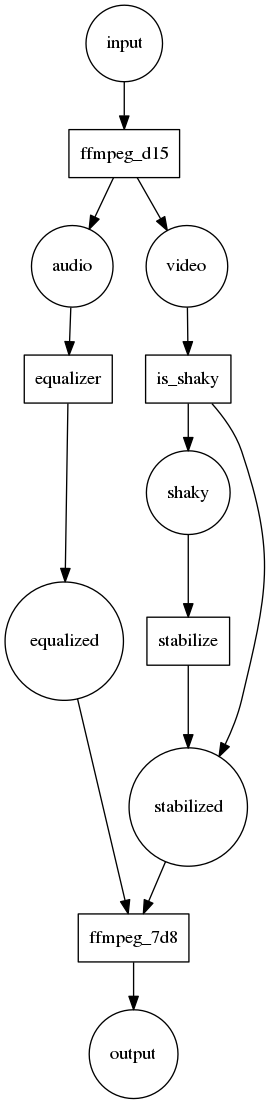
\includegraphics[width=.4\textwidth]{whole_pipeline.pdf}
\end{center}
\caption{The new pipeline, with branching and merging.}
\label{fig:whole}
\end{figure}


% \subsection{Weighted arcs}

\section{Tooling}
Because {\tt pmjq} relies on the filesystem and on users and groups, the standard UNIX tooling can easily manage the creation, installation, running and cleaning of advanced pipelines.

Files (\emph{tokens}) in a directory (\emph{place}) can be counted with {\tt ls <dir> | wc -l}.

Because {\tt pmjq} instances are launched in {\tt launch.sh} with {\tt sudo -u pu\_something pmjq ...}, one can find the active processes for a given transition with {\tt sudo -u pu\_something ps -A}.

All user names are prefixed with {\tt pu\_}, and all groups with {\tt pg\_}, therefore one can kill all the {\tt pmjq} processes by running :
{\tt \small
\begin{verbatim}
cat /etc/passwd | cut -d: -f1 | grep -E '^pu_'\
 | xargs -I user sudo -u user ps -A | cut -d' '\
 -f1 | kill -9
\end{verbatim}
}

The processes writing or reading from a directory can be listed with {\tt lsof}, resource usage can be monitored using {\tt top}, logs emitted by {\tt pmjq} can be greped, logrotated, syslogded, etc.

Multiple simulation tools exists that can be leveraged to simulate, and find the statistical properties of a given Petri Net, without having to actually run the associated, potentially resource-intensive {\tt pmjq} pipeline. Log analysis can provide data about the transition probabilities, the mean waiting time, etc. In our example pipeline, one could determine if the {\tt is\_shaky} branching is worth the trouble by searching for the probability of a token to take one branch or the other, and by measuring the delay induced by the {\tt is\_shaky} transition.

\section{Fault-Tolerance}

If the underlying filesystem is persistent, and provided transitions are idempotent and an integrity mechansim is in place\endnote{Such as appending the hash of the data to the filenames.}, all active processes can be brutally killed, and then {\tt launch.sh} can be run again to restart the processes, without any adverse effect. One can even change the topology before launching again.

Loud failure of one command will not crash the pipeline, but will simply cause files to accumulate in its input directory(ies). The rest of the pipeline will keep on running while the admins troubleshoot the problem. In our example (\autoref{fig:whole}), a bug in the {\tt equalizer} program would probably be only a minor inconvenience. Because video processing is so resource intensive, the computer(s) will stay busy running {\tt is\_shaky} and {\tt stabilize} while the progammers remove the bug in {\tt equalizer}. When it is launched back up, the files that have accumulated in {\tt audio} will be processed.

Silent failure and data corruption can not be mitigated by {\tt pmjq} alone, of course. Therefore it is important to fail loudly and as soon as possible.

\section{FileSystem choice matters}
Compromises can be made between security, fault-tolerance and speed. RAM filesystems are great for speed, but a computer crash will cause data loss. Encrypted disks are very secure, but performance may become an issue, etc.

The performance of {\tt pmjq} will be strongly tied to the performance of the underlying file system.

There has been decades of research on File Systems, and once performance becomes an issue one has to carefully weigh a lot of criteria (safety, security, performance, cost, maintanability, etc.). Here is an incomplete list of File Systems, OS or tools that can be useful in conjunction with {\tt pmjq} :
\begin{itemize}
\item Distributed File Systems
  \begin{itemize}
  \item GlusterFS \url{https://www.gluster.org/}
  \item SeaweedFS \url{https://github.com/chrislusf/seaweedfs/}
  \item HDFS \url{https://hadoop.apache.org/docs/r1.2.1/hdfs_design.html}
  \end{itemize}
\item Versionned File Systems
  \begin{itemize}
  \item GitFS \url{https://www.presslabs.com/gitfs/}
  \item Fossil~\cite{fossil}
  \end{itemize}
\item Others
  \begin{itemize}
  \item Plan 9 from Bell Labs \url{http://9p.io/plan9/index.html}
  \item FUSE \url{https://github.com/libfuse/libfuse}
  \item SSHFS \url{https://github.com/libfuse/sshfs}
  \item IPFS~\cite{ipfs}
  \end{itemize}
\end{itemize}

\section{Related works}
Easy and flexible parallel computing can be done with GNU Parallel (\url{https://www.gnu.org/software/parallel/}). 

Upgrading to full-grade concurrency necessitate the use of frameworks like 0MQ (whose manual \url{http://zguide.zeromq.org/page:all} is a great introduction to concurrency in general), RabbitMQ (\url{https://www.rabbitmq.com/}), Kafka (\url{https://kafka.apache.org/}), etc. All these systems are great and big projects are running thanks to them. They provide lots of features, and are well documented and battle-tested.

The most elegant alternative to {\tt pmjq} is Plan 9's plumber~\cite{plumber}, which, used whithin a Plan 9 cluster, will provide seamless concurency, strong authentication (with {\tt factotum}), and handle distribution without having to think about it. Showing that some carfully-constructed plumbing rules map to Petri Nets should not be too hard.

\section{Conclusion and further work}
We provide a proof-of-concept real-life implementation of a mathematically sound model of concurency (the Petri Nets) by having a daemon watch directories for files to process and write the output(s) in other directories. The implementation is very simple yet extremely powerful. Accompanying tools let the user intuitively design, visualize and manage complex systems.

The reliance on file systems and standard UNIX tools leverage the huge number of off-the-shelf sysadmin tools and the decades of research in distributed, fault-tolerant, secure file systems.

{\tt pmjq} is already used as a prototyping tool, and has yet to reach a point where the performance issues of the underlying filesystem negatively impact its usefulness. More formal tests are going to be run.

It is also a great tool for ungodly hacks, such as self-modifying topologies (which of course break the Petri Net model).

More work is expected to be done on the GUI front, most notably for real-time monitoring tools.

\section{Acknowledgments}

The author would like to thank his family for the support, his current employer (Gendarmerie Nationale) and its former employer (Sekoia) for letting him develop parts of {\tt pmjq} on duty/company time, and all the developers of free and open source software around the world for the many tools used to produce this paper.


\section{Availability}

{\tt pmjq} and the accompanying tool's source code is available at:

\begin{center}
{\tt https://github.com/edouardklein/pmjq }\\
\end{center}

Except where explicitely specified in the paper, all the mentioned features are implemented and tested. There will be a small delay between the deadline for the submission and the uploading of the version of {\tt pmjq} that we used to write this paper.

{\footnotesize \bibliographystyle{acm}
\bibliography{main}}


\theendnotes

\end{document}






